\chapter{Dataset}\label{sec:dataset}

\section{Data Collection}
In this work, we will use the data generated by the tracking systems of Digitec Galaxus AG.
The following sequence-diagram provides an overview of the data collection process.
\begin{figure}[H]
	\centering
    \captionsetup{width=0.8\textwidth}
    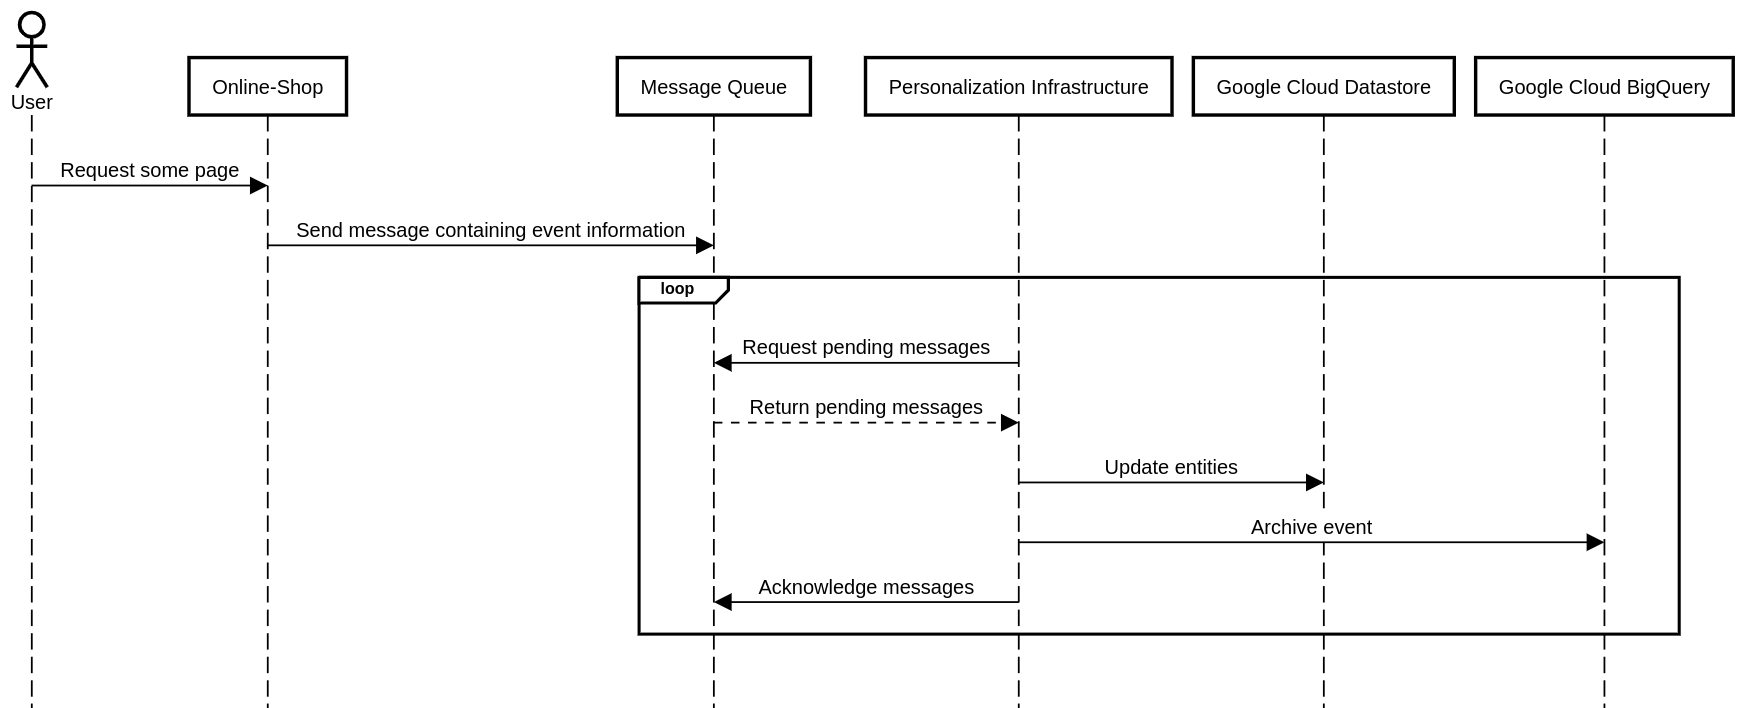
\includegraphics[width=\textwidth]{collecting-data.png}
    \caption{Collecting user interaction data on digitec.ch and galaxus.ch}
    \label{fig:collecting_data}
\end{figure}
When a user requests a specific page, the online shop Application will collect some information on the user such as UserId, requested page, User Agent.
This information is packaged as a message representing this specific event and then sent to a message queue.
Subsequently the Personalization Infrastructure will process these events by requesting batches of unprocessed messages.
For each event then the Personalization Infrastructure will first update the involved entities and then archive the event.
In the former case a managed Key-Value store (Google Cloud Datastore) is used to store entities.
Examples of such entities are shopping carts, orders, and last viewed products.
These entities basically represent the current state of various entities appearing in the context of the online shop.
In the latter case, a managed data warehousing solution (Google BigQuery) is used in order to be able to store large amounts of data in append-only tables.
The data stored there is mainly denormalized, in order to enable simple extraction.
Each row in these append-only tables contains all information belonging to a single event produced by a user.
The data stored in the Key-Value store essentially is the sum of all events stored in the data warehouse.

\section{Data Preparation}
In order to be able to focus on the model implementation when implementing the model, we want to prepare the data for congestion as far as possible.
Therefore, the extraction and preparation of the dataset is implemented separately from the model implementation.
\paragraph{Data Extraction}
In the first step, we extract the raw data from the data warehouse, selecting the following pieces of information: ProductId, LastLoggedInUserId, UserId, SessionId, User Agent, Timestamp.
Most of the properties are self-explanatory, except LastLoggedInUserId.
This property represents the UserId last seen on a specific device accessing the online shop.
When not actively logged into the accout, we would not know which accessed the page.
However, using this property, we can complete missing UserIds in the dataset.
The data extracted is limited to the events producted by visiting a product detail page as seen in figure~\ref{fig:product_detail}.
This filtering is done because this work focuses on recommending products, in another setting, other data might also be relevant.
The extracted data is stored in several shards of CSV files, each shard approximately represents the events of one day.
\begin{figure}[t]
	\centering
	\captionsetup{width=0.8\textwidth}
    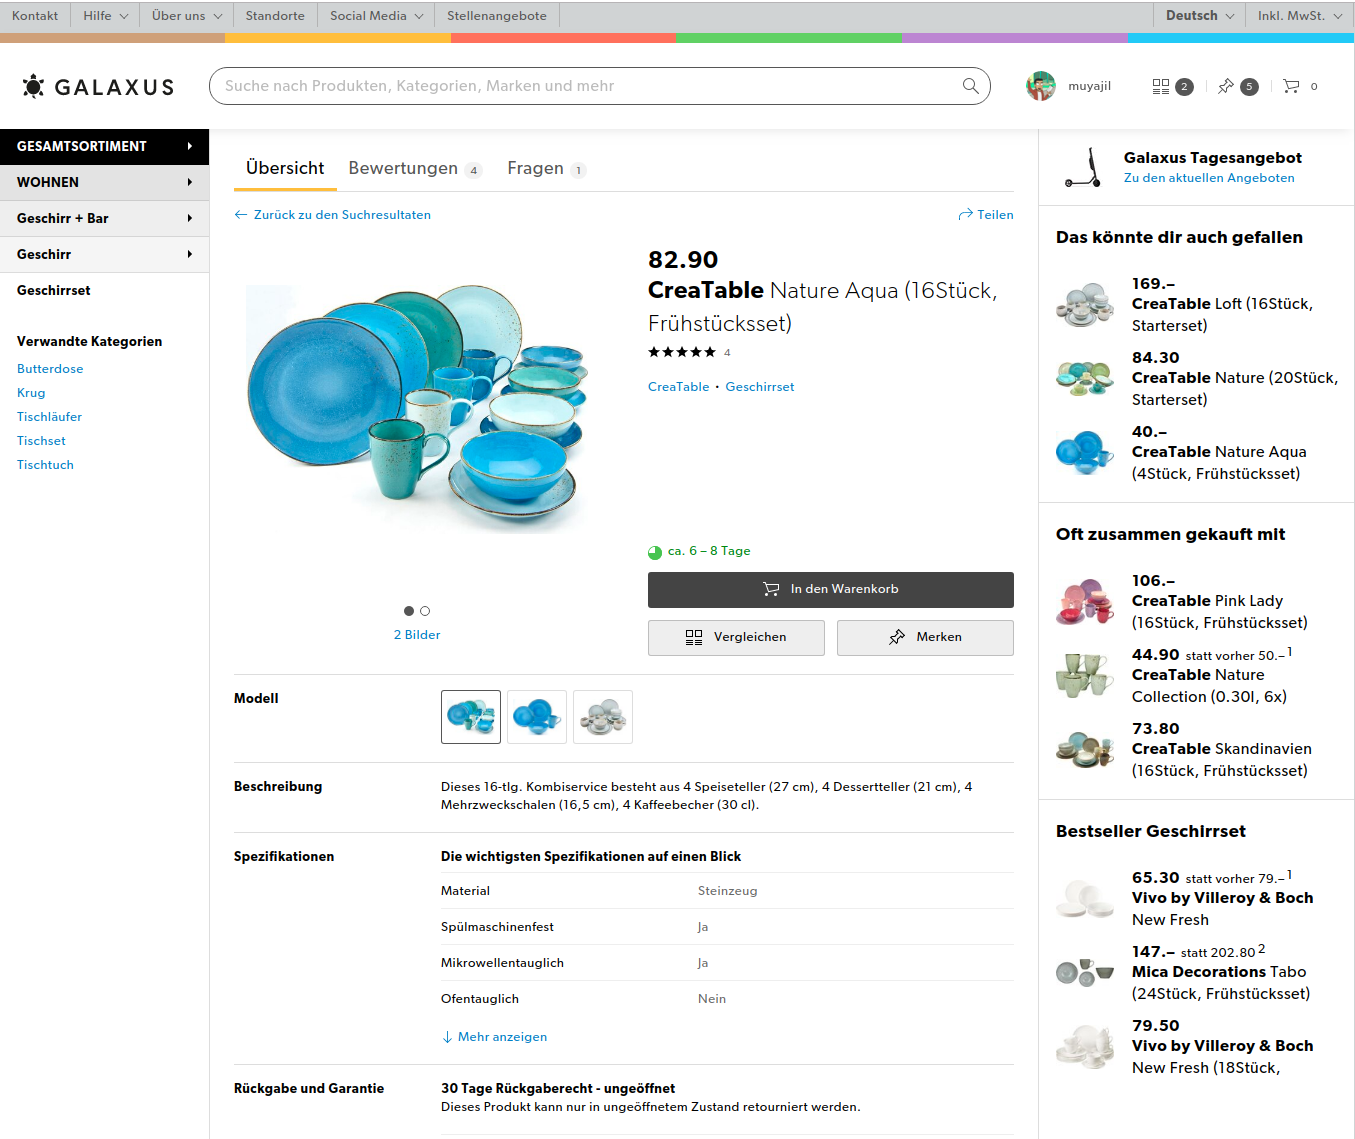
\includegraphics[width=\textwidth]{product-detail.png}
    \caption{Product Detail Page on galaxus.ch}
    \label{fig:product_detail}
\end{figure}
\paragraph{Cleaning Data}
In the next step, the data is cleaned, which involves mainly two steps:
Anytime we encounter an event where the user is unkown, we try to complete the information with the LastLoggedInUserId. 
If we do not know the LastLoggedInUserId either we discard the event.
\par
There are many well-known bots roaming the internet collecting various types of information on websites.
Most famously the Google Bot which crawls the content of any website to determine the quality of the site and to influence the rank of the website in Google searches.
There are some open-source lists that collect the User Agents of these bots.
The User Agent of a client accessing a website usually describes the type of device used, in the case of "good" bots, they explicitly tell the server that the "device" accessing the website is actually a bot.
Using one of these lists\footnote{\url{https://raw.githubusercontent.com/monperrus/crawler-user-agents/master/crawler-user-agents.json}} the events produced by bots are removed from the dataset.

\paragraph{Aggregation of Events}
The next step is to aggregate the events on two levels: first grouping events that were generated in the same session and second grouping these sessions by users.
The resulting data structure looks as follows:

\begin{minipage}{\linewidth}
    \begin{lstlisting}[language=Python,frame=single,caption=Data Structure for user-events,label=code:user-events]
    "<UserId_1>": {
        "<SessionId_1>": {
            "StartTime": "<Timestamp of first event>",
            "Events": [
                {
                    "ProductId": "<ProductId_1>",
                    "Timestamp": "<Timestamp_1>"
                },
                {
                    "ProductId": "<ProductId_2>",
                    "Timestamp": "<Timestamp_2>"
                }
            ]
        }
    }
    \end{lstlisting}
\end{minipage}
This is done by processing one shard after another; when a shard is finished, the JSON representation of this shard is saved in a separate file because the large amount of datapoints cannot be kept in memory altogether.
\paragraph{Merging shards}
Since the shards only approximate the events of one day, it is not possible to assume that a session is completely represented in one shard, it might be distributed across multiple.
Therefore, it is necessary to merge the data in the different shards, but since it is not efficient to keep all the information in one file, a different method of paritioning is required.
As we will see later, it is further necessary that all the events produced by a single user are stored in the same file.
An easy way of achieving this, is by partitioning by UserId.
Each shard is processed as follows:

\begin{minipage}{\linewidth}
    \begin{lstlisting}[language=Python,frame=single,caption=Merging shards,label=code:merging-shards]
    for shard in shards:
        for i in range(num_target_files):
            relevant_user_ids = list(filter(lambda x: int(x) % num_target_files == i, shard.keys()))
            output_path = merged_shards_prefix + str(i) + '.json'
            output_file = json.load(output_path)
            for user_id in relevant_user_ids:
                for session_id in shard[user_id]:
                    # Merge events from output_file and shard
    \end{lstlisting}
\end{minipage}
\paragraph{Filtering}
Having some number of files containing all the information relevant to some users, some datapoints have to be filtered out, which is also mentioned by the authors of~\cite{hierarchical}.
Specifically the following:
\begin{itemize}
    \item Remove items with low support (min 5 events per product)
    \item Remove users with few sessions (min 5 sessions per user)
    \item Remove sessions with few events (min 3 events per session)
\end{itemize}
Those datapoints are removed since items with few interactions are suboptimal for modeling; too short sessions are not informative, and finally users with few sessions produce few cross-session information.

\paragraph{Subsampling}
Prototyping models with very large datasets is inefficient.
Therefore, several different sizes of the dataset were produced, by defining the approximate number of users and the exact number of products desired in the dataset.
This was done by sampling from the set of products with a probability proportional to the number of events on that product.
Subsequently, the partitions of the data were processed, iterating through the sessions of the users.
For each sessions we remove the products that were not chosen to be kept and keep the session if it is still long enough.
Furthermore, a user is kept in the dataset if the number of filtered sessions remains still large enough.
This process is repeated for the different partitions until the number of users is larger than the approximate number of desired users.

\paragraph{Embedding Dictionary}\label{sec:embedding_dict}
As we will see in~\ref{sec:model_arch}, a version of the model uses one-hot encodings for representing products.
Therefore, the product IDs referenced in the dataset need to be mapped into a continuous ID space, otherwise it is not possible to produce one-hot encodings.
The process starts with EmbeddingId 0, then iterates through all the sessions, and each time a product is seen for the first time, the EmbeddingId is assigned to the product increased by 1.

\section{User Parallel Batches}
Since we are dealing with sequence data, it is not trivial to produce batches for the model to ingest.
Because the sequences can have different lengths, and the number of sessions varies from user to user.
User Parallel Batching is a way of having fixed size batches that can be ingested by the model, while allowing for sequences to have different lengths and users to have a different number of sessions.
Usually, in these cases the sequences are padded with some neutral value, however in this case, there is no neutral product, and the introduction of such a neutral product might influence the results.
When processing sequence data, it usually means that a datapoint is the input for the next datapoint, which requires the ordered sequence data.
To illustrate these batches, we assume that there are 4 users with the sessions as in figure~\ref{fig:user_parallel_batches}.
\begin{figure}[t]
	\centering
	\captionsetup{width=0.8\textwidth}
    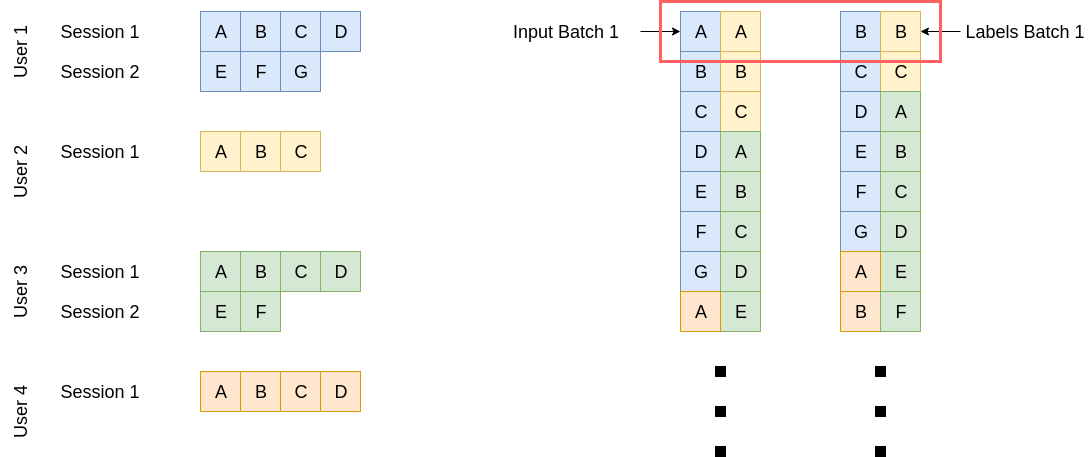
\includegraphics[width=\textwidth]{user_parallel_batches.png}
    \caption{User Parallel Batches}
    \label{fig:user_parallel_batches}
\end{figure}
A batch of size $x$ will contain an event from $x$ different users.
Essentially, the labels are the event that happens after the input event.
\par
The data representation shown in listing~\ref{code:user-events} is chosen explicitly to enable efficient generation of user parallel batches.
To compute the loss function mentioned in~\ref{sec:hgru4rec}, we sample the irrelevant items by using the items from the different sessions in the same batch.
This basically enables popularity based sampling, since the samples are directly taken from other sessions.

\section{Dataset Properties}\label{sec:dataset_properties}
Using the afromentioned sampling step, we generated different sizes of the dataset to enable model prototyping.
In table~\ref{tab:dataset_stats}, we can see the properties of the different datasets.
\begin{table}[t]
    \centering
    \begin{tabular}{lrrr}\toprule
        \textbf{Property} & \textbf{MINI Dataset} & \textbf{MIDI Dataset} & \textbf{MAXI Dataset} \\ \midrule
        \#Users & 23 & 15'242 & 242'797 \\
        \#Products & 161 & 42'103 & 470'817 \\
        \#Events & 633 & 1'234'697 & 28'726'701 \\
        \#Sessions & 183 & 250'187 & 4'652'496 \\ \midrule
        \#Events per Product & 3.93 $\pm$ 5.84 & 29.33 $\pm$ 69.98 & 61.27 $\pm$ 263.3 \\
        \#Events per User & 27.52 $\pm$ 19.8 & 81.01 $\pm$ 135.35 & 115.05 $\pm$ 215.15 \\
        \#Events per Session & 3.46 $\pm$ 0.82 & 4.94 $\pm$ 3.07 & 6.17 $\pm$ 60.22 \\ 
        \#Sessions per User & 7.96 $\pm$ 5.41 & 16.41 $\pm$ 22.08 & 19.16 $\pm$ 28.67 \\ \bottomrule
    \end{tabular}
    \caption{Dataset Properties}
    \label{tab:dataset_stats}
\end{table}
The MINI dataset is used to ensure that the model works. 
The goal is to completely overfit to the training data and remember everything, which allows to quickly debug and validate the gradient flow through the model.
The MIDI dataset is used for experiments with different model sizes.
The purpose of this dataset is to try out different models on a rather realistic dataset, which is of similar size than the ones used in~\cite{hierarchical}, and to be able to train these models in a reasonable time frame.
The MAXI dataset on the other hand, contains all events that were not filtered in the data preparation process.
Depending on the model size, training on this dataset can take several days, which is why only the models that performed best on the MIDI dataset were trained on the MAXI dataset.
Finally, the models that are deployed in the experiments are all trained on the MAXI dataset.